\documentclass[twocolumn,english]{IEEEtran}
\usepackage[T1]{fontenc}
\usepackage{babel}
\usepackage{amsthm}
\usepackage{amsmath}
\usepackage{graphicx}
\usepackage[unicode=true,
 bookmarks=true,bookmarksnumbered=true,bookmarksopen=true,bookmarksopenlevel=1,
 breaklinks=false,pdfborder={0 0 0},backref=false,colorlinks=false]
 {hyperref}
\usepackage{bm}
\usepackage{amsmath}
\usepackage{amssymb}
\usepackage{natbib}
\usepackage{array}
\usepackage{calc}
\newcommand{\vb}[1]{\mathbf{#1}}		%Bold vector
\newcolumntype{W}{>{\centering\arraybackslash}m{25mm}}
\newcolumntype{L}{>{\centering\arraybackslash}m{15mm}}
\usepackage{booktabs}

%%%%%%%%%%%%%%%%%%%%%%%%%%%%%%%%%%%%%%%%%%%%%%%%%%%%%%%%%%%%%%%%%%%%%%%%%%%%%%% Variables
\newcommand{\thetitle}{Project 4: Survey and Analysis}
\newcommand{\theauthors}{Zack Garza}
\newcommand{\theclass}{Math 142: Elementary Statistics}
%%%%%%%%%%%%%%%%%%%%%%%%%%%%%%%%%%%%%%%%%%%%%%%%%%%%%%%%%%%%%%%%%%%%%%%%%%%%%%%%%%%%%%%%%%

\hypersetup{
 pdftitle=  {\thetitle},
 pdfauthor= {\theauthors},
 pdfpagelayout=OneColumn, pdfnewwindow=true, pdfstartview=XYZ, plainpages=false}

\makeatletter


%%%%%%%%%%%%%%%%%%%%%%%%%%%%%% Textclass specific LaTeX commands.
 % protect \markboth against an old bug reintroduced in babel >= 3.8g
 \let\oldforeign@language\foreign@language
 \DeclareRobustCommand{\foreign@language}[1]{%
   \lowercase{\oldforeign@language{#1}}}
\theoremstyle{plain}
\newtheorem{thm}{\protect\theoremname}
\theoremstyle{plain}
\newtheorem{lem}[thm]{\protect\lemmaname}

%%%%%%%%%%%%%%%%%%%%%%%%%%%%%% User specified LaTeX commands.
% for subfigures/subtables
\ifCLASSOPTIONcompsoc
\usepackage[caption=false,font=normalsize,labelfont=sf,textfont=sf]{subfig}
\else
\usepackage[caption=false,font=footnotesize]{subfig}
\fi

\makeatother
\providecommand{\lemmaname}{Lemma}
\providecommand{\theoremname}{Theorem}
\setcounter{topnumber}{2}
\setcounter{bottomnumber}{2}
\setcounter{totalnumber}{4}
\renewcommand{\topfraction}{0.85}
\renewcommand{\bottomfraction}{0.85}
\renewcommand{\textfraction}{0.15}
\renewcommand{\floatpagefraction}{0.7}
\usepackage{float}
\onecolumn

\usepackage{Sweave}
\begin{document}

\title{\thetitle}
\author{\theauthors}
\IEEEspecialpapernotice
{\theclass \\ Effective Date of Report: \today }
\markboth{\thetitle}{\theauthors}
\maketitle
\tableofcontents


\hrulefill

\section{Theme}
\IEEEPARstart{T}he 



\newpage




\section{Description}
Lunch: K-12 Students Eligible for Free and Reduced Priced Meals (FRPM), reported by schools in 2012.
STAR Scores: The Mean Scale Score across all STAR subject tests given to K-12 students.
\subsection{Population and Sample}
\subsection{Sampling Technique}

To begin with, both data sets were downloaded, and extraneous results (such as state-wide or county-wide tallies) were filtered out. 
The remaining data described 8562 schools in 1575 disricts, distributed among 58 counties in California. 

The average number of schools per county was around 150, meaning that there was over a 97\% chance that selecting any county would result in a sample size greater than 30. 
Thus, this method provided a very high probability of fulfilling the requirement of $n \geq 30$ required for many of the following statistical analyses.

To select two independent populations, two counties were selected at random.

From the two chosen counties, simple random samples of 50 schools were taken without replacement from all of the districts and schools within that county.

From this data, a list of unique school codes were generated. 
This allowed cross-referencing the primary data sets.






\subsection{Survey Questions}

The schools codes were matched up with the STAR scores in the first data set, and the reduced/free lunch statistics in the second data set. 
This essentially amounted to "querying" the two samples in the following ways:

\begin{itemize}
		\item \textbf{Quantitative}:

				What was the average STAR score among K-12 students at this school?

				What proportion of this school's student population qualifies for free or reduced lunch?
		\item \textbf{Qualitative}:

				What were the students' parental education levels at this school?
\end{itemize}






\section{Data and Analysis}

\begin{figure}[H]
\begin{centering}
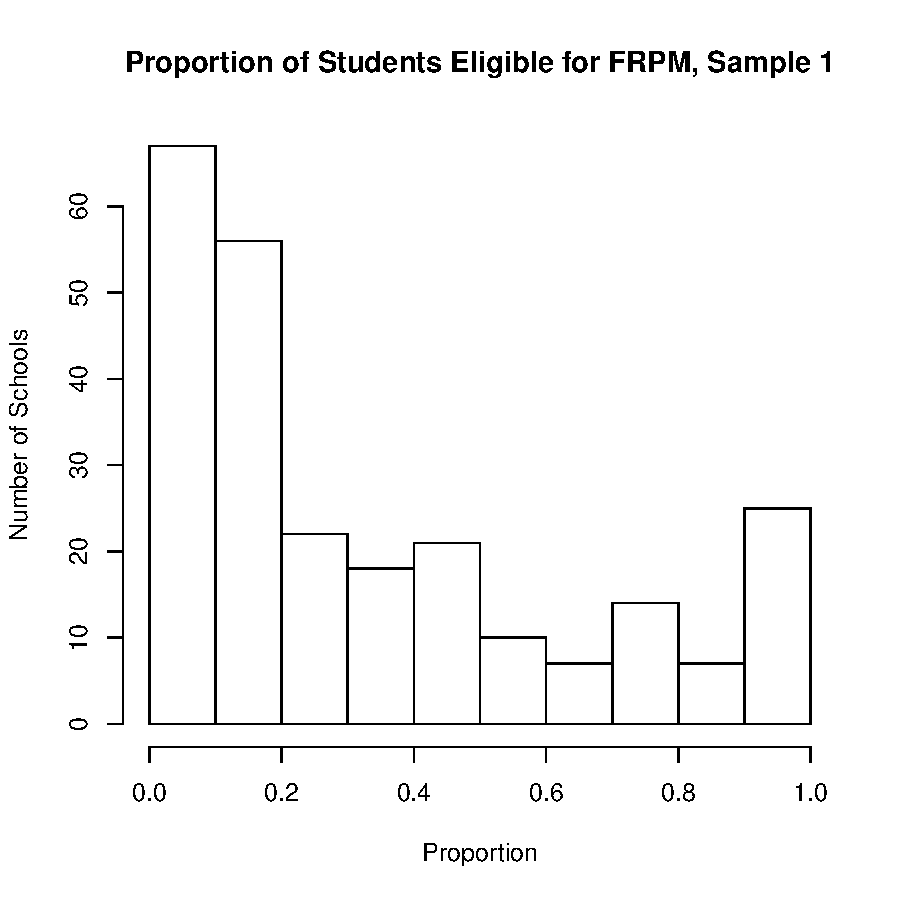
\includegraphics{proj3-fig_lunch_props2}
\caption{Proportions.}
\label{fig:Lunch_Hist_Two}
\end{centering}
\end{figure}



\begin{figure}[H]
\begin{centering}
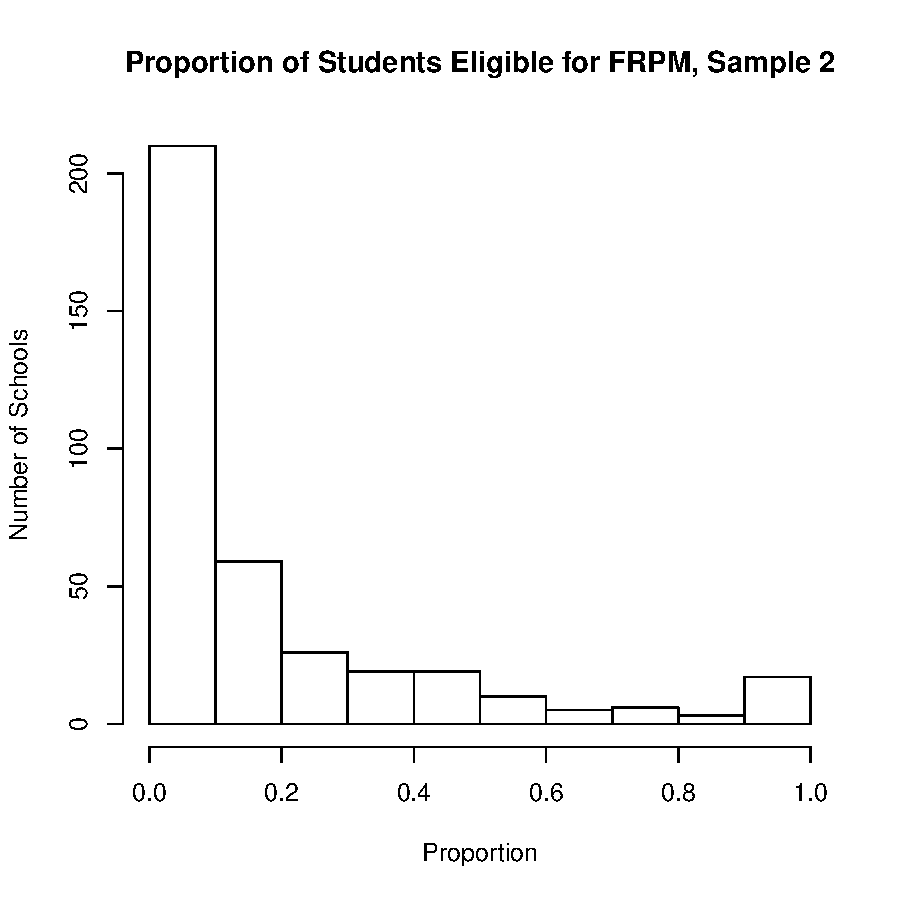
\includegraphics{proj3-fig_lunch_props1}
\caption{Proportions.}
\label{fig:Lunch_Hist_One}
\end{centering}
\end{figure}


% One Pie chart or pareto chart
% One frequency distribution: Frequency, Percentage Frequency, Cumulative Frequency. 5-8 Classes
% One histogram
% One Frequency Polygon
% One Ogive

% Summary statistics for both samples.
		% Size, mean, sd, sample variance, 5 number summary, range of usual values
% Two modified box plots (one for each)

% 95 percent confidence interval

% Hypothesis test with p values

\section{Conclusion}



%\bibliographystyle{plain}
%\bibliography{physbib}

\end{document}
